% !TeX root = document.tex
% !TeX encoding = UTF-8 Unicode

\chapter{PID}%
\label{chapter:pid}

\begin{mdframed}[frametitle={Atenção!}]
    A execução deste módulo se basea na existência de conexão entre o
    \textbf{Lachesis} e o \textbf{moirai}. Para parar a execução você deve
    navegar para um outro módulo. Os dados são atualizados a cada segundo mas
    apenas são aplicados quando o \textbf{moirai} os processar, o que pode levar
    mais de um tempo de amostragem, \textbf{inclusive para parar o teste}!

    \textbf{NÃO DEIXE ESTE MÓDULO EXECUTANDO SEM ESTAR POR PERTO E ATENTO!!!}
\end{mdframed}

Esse módulo, exibido na Figura~\ref{fig:pid} permite executar um controlador
PID, e a alterar os valores durante a execução. \textit{Entrada} e
\textit{Saída} são do ponto de vista do \textit{software}, ou seja,
\textit{Entrada} é um sensor e \textit{Saída} um atuador. \textit{Min} e
\textit{Max} definem os valores mínimo e máximo de saturação do atuador,
respectivamente.

\begin{figure}[ht!]
    \centering
    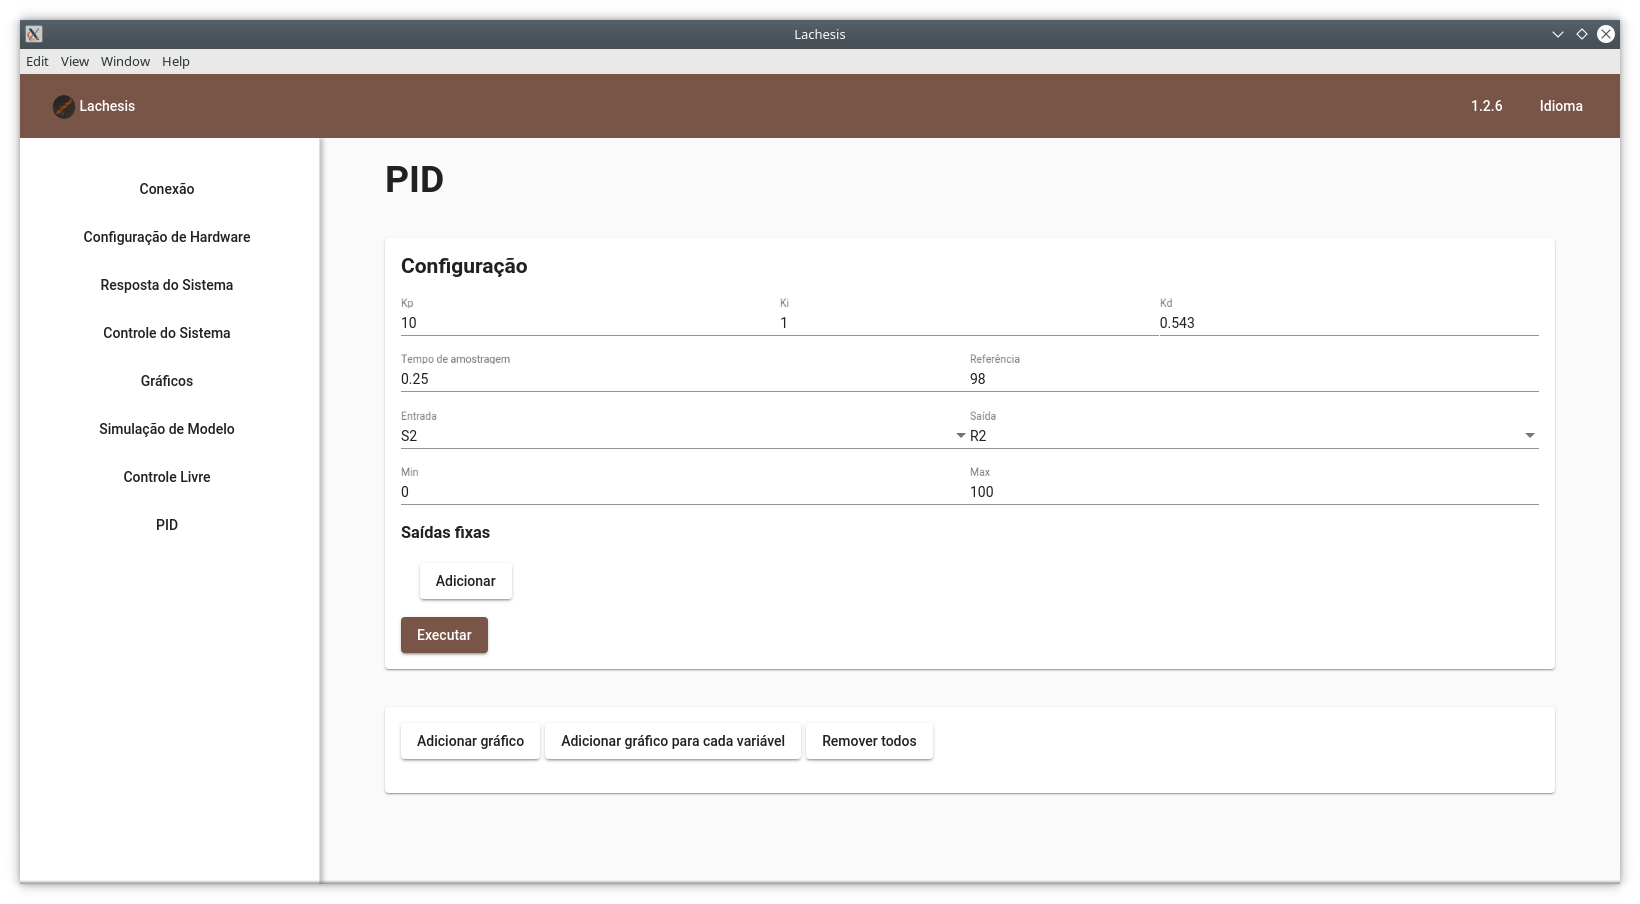
\includegraphics[width=0.9\textwidth]{imgs/pid}
    \caption[Módulo PID]{Módulo PID}%
    \label{fig:pid}
\end{figure}

Assim como em \textit{Controle Livre}, saídas fixas podem ser adicionadas e
modificadas durante o teste. Os atrasos nas atualizações de valores e detecção
de perda de conexão também ocorrem da mesma forma. Os dados também são salvos e
ficam disponíveis no módulo \textit{Gráficos}.
